% Figure LaTeX snippets for TEMPy-REFF paper. Not input-ed; embedded inline in main.tex.

\begin{figure}[t]
  \centering
  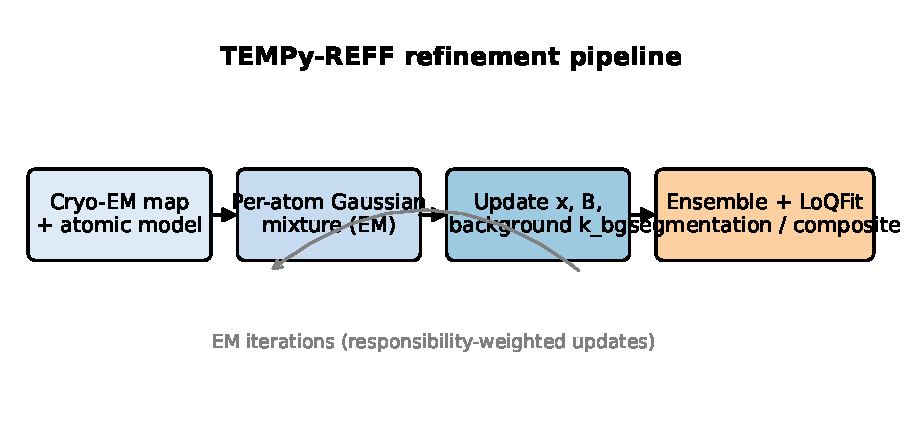
\includegraphics[width=0.7\linewidth]{figures/fig_pipeline_schematic.pdf}
  \caption{Overview of the TEMPy-REFF pipeline. A cryo-EM map and an initial atomic model are represented as a per-atom Gaussian mixture with a uniform background; responsibility-weighted expectation-maximisation jointly updates atomic positions $x$, per-atom B-factors $B$, and the background level $k_{\mathrm{bg}}$. The converged model supports ensemble generation, LoQFit scoring, and responsibility-weighted map segmentation or composition.}
  \label{fig:pipeline}
\end{figure}

\begin{figure}[t]
  \centering
  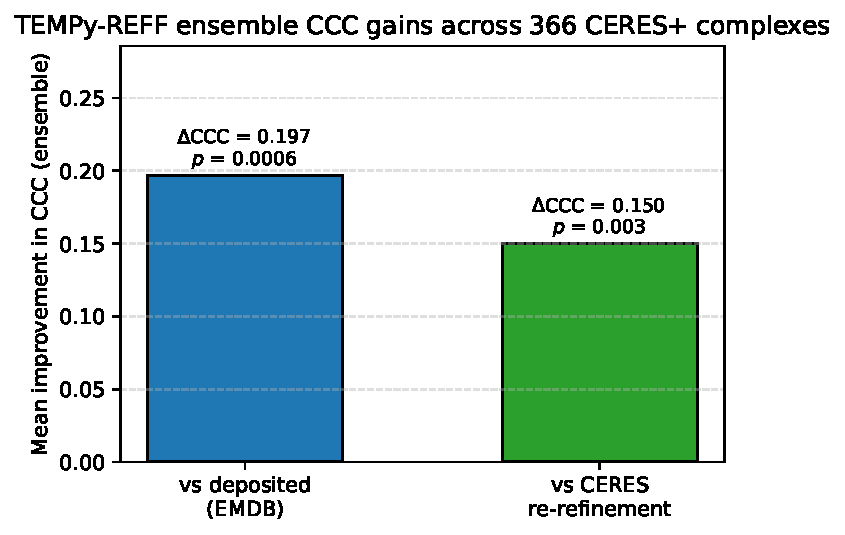
\includegraphics[width=0.65\linewidth]{figures/fig_ccc_delta.pdf}
  \caption{Mean improvement in ensemble cross-correlation (CCC) across the 366-complex CERES+ benchmark. Paired $t$-tests give $\Delta\mathrm{CCC}=0.197$ against deposited EMDB models ($p=0.0006$) and $\Delta\mathrm{CCC}=0.150$ against CERES re-refined models ($p=0.003$).}
  \label{fig:ccc_delta}
\end{figure}

\begin{figure}[t]
  \centering
  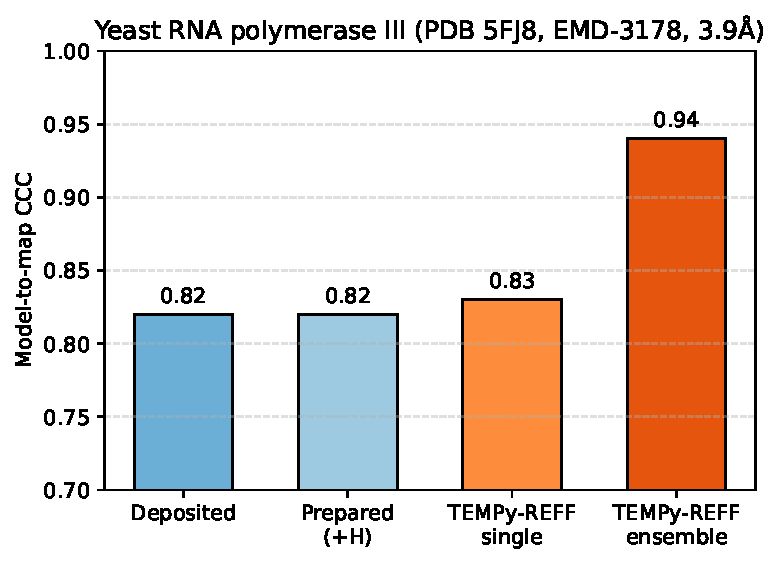
\includegraphics[width=0.7\linewidth]{figures/fig_rnapol_iii_ccc.pdf}
  \caption{Model-to-map cross-correlation for the yeast RNA polymerase III elongation complex (PDB 5FJ8, EMD-3178, 3.9~\AA). Deposited and hydrogen-prepared models both yield CCC~$=0.82$; TEMPy-REFF single-model refinement gives CCC~$=0.83$; the ensemble representation reaches CCC~$=0.94$.}
  \label{fig:rnapol_iii}
\end{figure}

\begin{figure}[t]
  \centering
  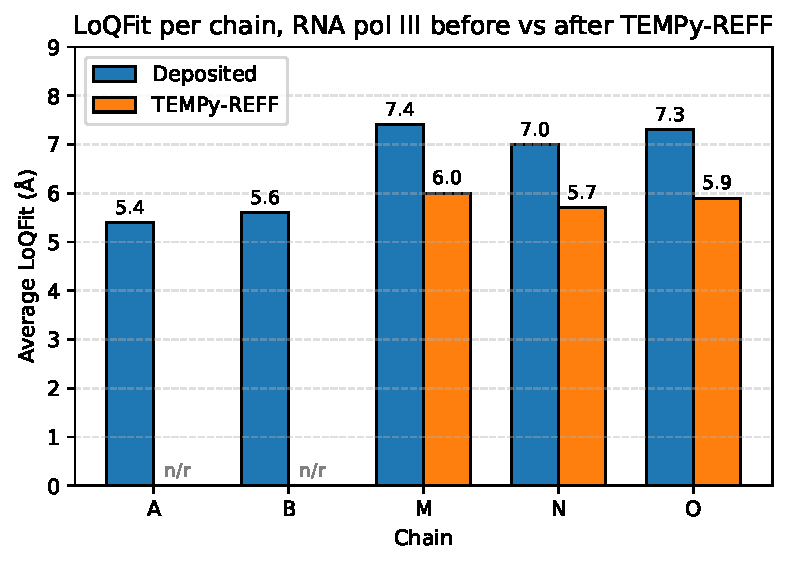
\includegraphics[width=0.75\linewidth]{figures/fig_loqfit_chains.pdf}
  \caption{Per-chain average LoQFit (\AA) for yeast RNA polymerase III before and after TEMPy-REFF refinement. Chains A and B lie in the well-resolved core (5.4 and 5.6~\AA, respectively; post-refinement values not reported individually). Solvent-exposed low-resolution chains M, N, and O improve from 7.4, 7.0, and 7.3~\AA\ to 6.0, 5.7, and 5.9~\AA.}
  \label{fig:loqfit_chains}
\end{figure}
